\documentclass[tikz,border=4mm]{standalone}
\usepackage[T1]{fontenc}
\usepackage{helvet}
\renewcommand{\familydefault}{\sfdefault}
\usetikzlibrary{arrows.meta,positioning,fit,backgrounds}

\begin{document}
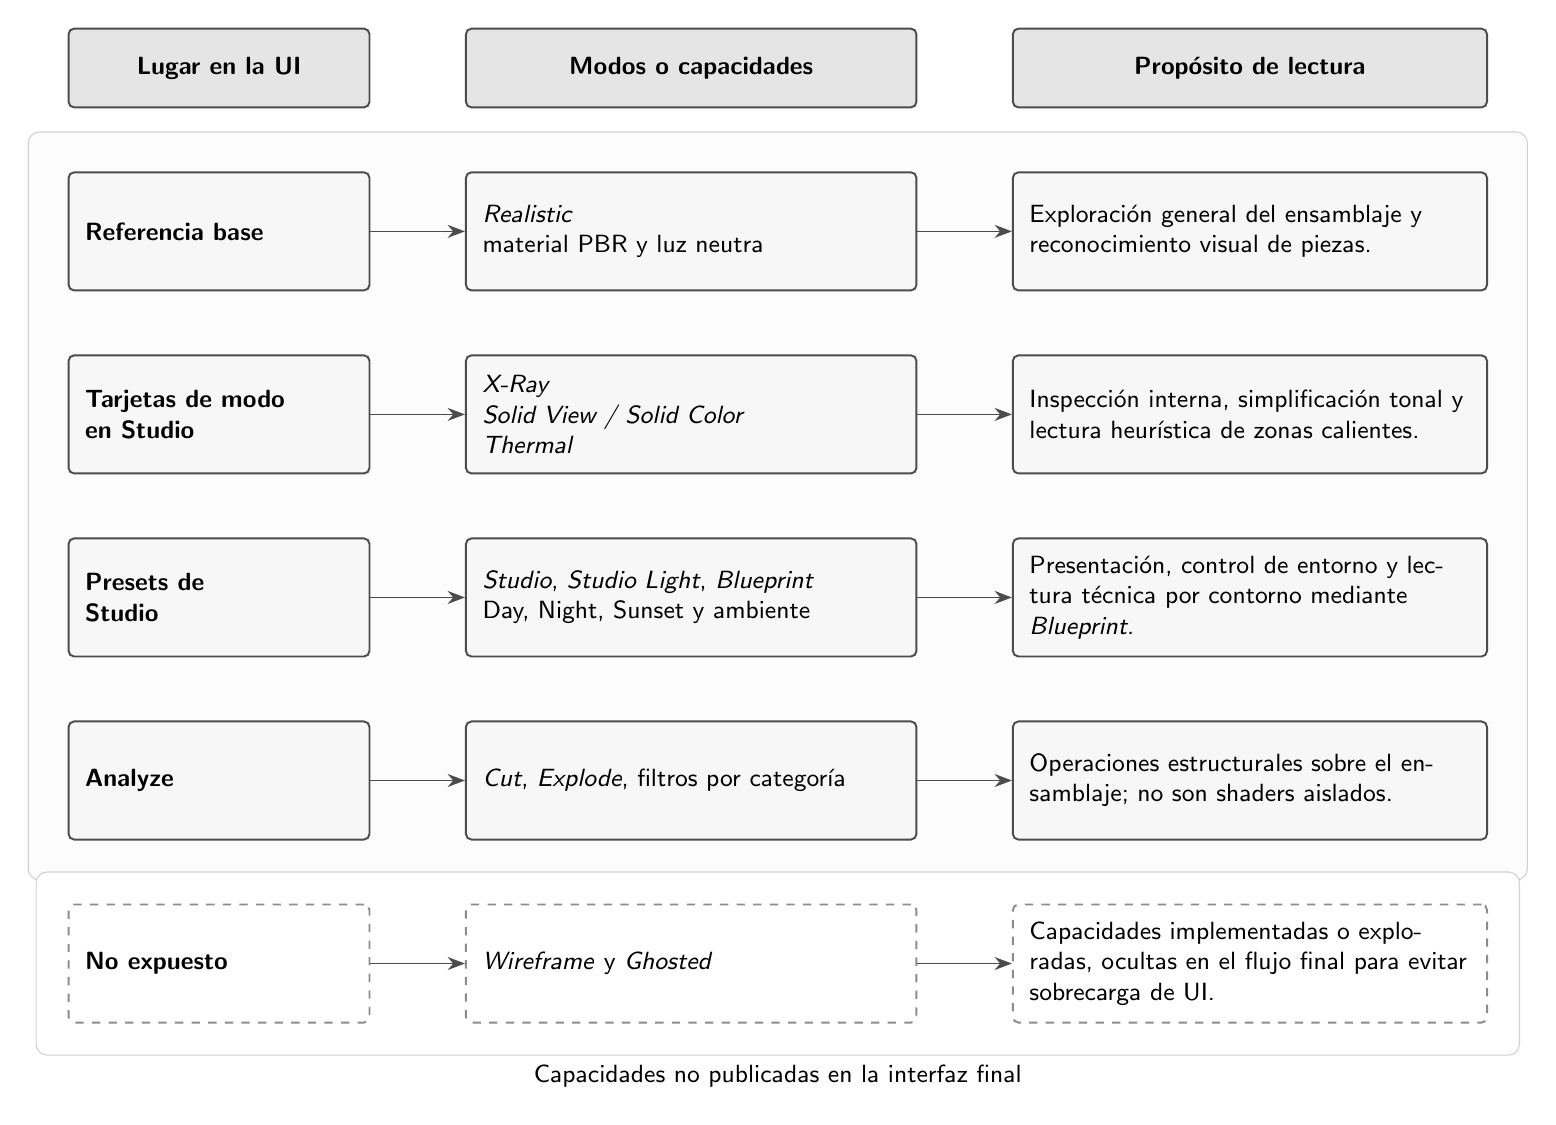
\begin{tikzpicture}[
  font=\sffamily\small,
  node distance=8mm and 12mm,
  box/.style={
    draw=black!70,
    rounded corners=2pt,
    line width=0.7pt,
    fill=black!3,
    align=left,
    inner sep=6pt,
    minimum height=15mm
  },
  head/.style={
    box,
    fill=black!10,
    align=center,
    font=\sffamily\bfseries\small,
    minimum height=10mm
  },
  group/.style={box, text width=34mm, font=\sffamily\bfseries\small},
  modes/.style={box, text width=53mm},
  purpose/.style={box, text width=56mm},
  hidden/.style={box, draw=black!45, fill=white, dashed},
  arrow/.style={-{Stealth[length=2.2mm]}, line width=0.62pt, draw=black!70}
]

\node[head, text width=34mm] (h1) {Lugar en la UI};
\node[head, text width=53mm, right=of h1] (h2) {Modos o capacidades};
\node[head, text width=56mm, right=of h2] (h3) {Prop\'osito de lectura};

\node[group, below=8mm of h1] (base) {Referencia base};
\node[modes, right=of base] (basemodes) {\textit{Realistic}\\material PBR y luz neutra};
\node[purpose, right=of basemodes] (basepurpose) {Exploraci\'on general del ensamblaje y reconocimiento visual de piezas.};

\node[group, below=of base] (shader) {Tarjetas de modo\\en \textit{Studio}};
\node[modes, right=of shader] (shadermodes) {\textit{X-Ray}\\\textit{Solid View / Solid Color}\\\textit{Thermal}};
\node[purpose, right=of shadermodes] (shaderpurpose) {Inspecci\'on interna, simplificaci\'on tonal y lectura heur\'istica de zonas calientes.};

\node[group, below=of shader] (studio) {Presets de\\\textit{Studio}};
\node[modes, right=of studio] (studiomodes) {\textit{Studio}, \textit{Studio Light}, \textit{Blueprint}\\Day, Night, Sunset y ambiente};
\node[purpose, right=of studiomodes] (studiopurpose) {Presentaci\'on, control de entorno y lectura t\'ecnica por contorno mediante \textit{Blueprint}.};

\node[group, below=of studio] (analyze) {\textit{Analyze}};
\node[modes, right=of analyze] (analyzemodes) {\textit{Cut}, \textit{Explode}, filtros por categor\'ia};
\node[purpose, right=of analyzemodes] (analyzepurpose) {Operaciones estructurales sobre el ensamblaje; no son shaders aislados.};

\node[group, hidden, below=of analyze] (internal) {No expuesto};
\node[modes, hidden, right=of internal] (internalmodes) {\textit{Wireframe} y \textit{Ghosted}};
\node[purpose, hidden, right=of internalmodes] (internalpurpose) {Capacidades implementadas o exploradas, ocultas en el flujo final para evitar sobrecarga de UI.};

\draw[arrow] (base) -- (basemodes);
\draw[arrow] (basemodes) -- (basepurpose);
\draw[arrow] (shader) -- (shadermodes);
\draw[arrow] (shadermodes) -- (shaderpurpose);
\draw[arrow] (studio) -- (studiomodes);
\draw[arrow] (studiomodes) -- (studiopurpose);
\draw[arrow] (analyze) -- (analyzemodes);
\draw[arrow] (analyzemodes) -- (analyzepurpose);
\draw[arrow] (internal) -- (internalmodes);
\draw[arrow] (internalmodes) -- (internalpurpose);

\begin{scope}[on background layer]
  \node[draw=black!18, rounded corners=4pt, fill=black!1,
    fit=(base)(basepurpose)(analyze)(analyzepurpose),
    inner sep=5mm] {};
  \node[draw=black!18, rounded corners=4pt, fill=white,
    fit=(internal)(internalpurpose),
    inner sep=4mm,
    label={[font=\sffamily\small]below:Capacidades no publicadas en la interfaz final}] {};
\end{scope}

\end{tikzpicture}
\end{document}
